\section{DICOM en pratique}

\frame
{
	\frametitle{Anonymisation}
	\begin{itemize}
		\item Utilisation d'images cliniques pour la recherche ou l'enseignement.
		\item<2-> Fichiers mis \`a disposition du public.
		\item<3-> N\'ecessit\'e d'anonymat : suppression des informations personnelles permettant d'identifier le patient.
		\begin{itemize}
			\item<4-> PatientsName (0010,0010)
			\item<5-> PatientID (0010,0020)
			\item<6-> PatientBirthDate (0010,0030) $\rightarrow$ de type 1 : \`a remplacer, pas supprimer !
			\item<7-> ReferringPhysicianName (0008,0090)
			\item<7-> etc.
			\item<8-> Potentiellement plus de 250 champs \`a supprimer ou \`a vider !
		\end{itemize}
	\end{itemize}
}

\frame
{
	\frametitle{DICOM Conformance Statement}
	\begin{itemize}
		\item Document pr\'ecisant le niveau de conformit\'e d'un produit (e.g. modalit\'e, logiciel, etc.) \`a la norme DICOM.
		\item<2-> Plan et structure pr\'ed\'efinis par la norme.
		\item<3-> Tr\`es technique :
		\begin{itemize}
			\item<4-> Diagrammes des flux de donn\'ees.
			\item<5-> Liste des services fournis.
			\item<6-> Liste des SOP Class support\'ees et des r\^oles assur\'es (SCU, SCP).
		\end{itemize}
	\end{itemize}
}

\frame
{
	\frametitle{Achat d'un \'equipement}
	\begin{enumerate}
		\item Avant l'achat, soumission de l'appel d'offre :
		\begin{itemize}
			\item<2-> D\'efinition du sc\'enario de travail souhait\'e.

			Exemple : les images brutes export\'ees pourront \^etre r\'eutilis\'ees \emph{a posteriori}.
			\item<3-> R\'edaction du cahier des charges DICOM.
			\begin{itemize}
				\item<3-> Pr\'eciser le niveau d'exigence de DICOM.
				
				$\rightarrow$ faire appel \`a un consultant ou \`a des coll\`egues,
				
				$\rightarrow$ ou acqu\'erir le savoir-faire en interne.
				\item<4-> Demander le DICOM Conformance Statement.
			\end{itemize}
		\end{itemize}
		\item<5-> Acceptation protocol\'ee.
		\begin{itemize}
			\item<6-> V\'erification de la correspondance entre DICOM Conformance Statements.
			\item<7-> V\'erification des sc\'enarios requis.
			\item<8-> Tests.
		\end{itemize}
	\end{enumerate}
}

\frame
{
	\frametitle{Services \`a demander}
	Exemples de services DICOM \`a exiger pour un scanner :
	\begin{itemize}
		\item<2-> Worklist (SCU)
		\item<3-> MPPS (SCU)
		\item<4-> Store (SCU)  : modalit\'e  \textbf{CT}
		\item<5-> R\'eception (SCP) : \textbf{CT}, \textbf{IRM}.
		\item<6-> Storage Commitment (SCU).
	\end{itemize}
	
	\begin{center}
		\includegraphics<7->[width=\linewidth]{./figures/services-ct.png}
	\end{center}
}

\frame
{
	\frametitle{\'Equipements non standards}
	
	\begin{itemize}
		\item Int\'egration possible dans un workflow DICOM via une passerelle de conversion.
		
		\begin{center}
			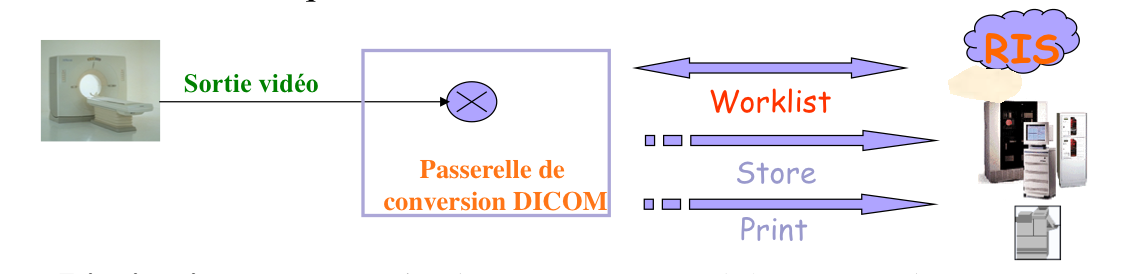
\includegraphics[width=\linewidth]{./figures/passerelle.png}
		\end{center}
		\item Limitation : images stock\'ees en mode Secondary Capture (IOD le plus simple de DICOM), les donn\'ees d'acquisition des images sont perdues.
	\end{itemize}
}

